In this section we first motivate our microservice approach based on our
experiences developing the MIxT web application.
We describe the process from initial data analysis to the final application,
highlighting the importance
% LAB + performance/scalability/deployment (dvs noe som er kvantifiserbart)
of language-agnostic services to facilitate the use of different tools in
different parts of the application. 
%This is especially important in
%interdisciplinary teams where researchers use a wide range of tools and
%programming languages.  
%We believe many systems biology data exploration applications are developed
%similarly and that they can therefore also benefit from the microservice
%approach. 
Based on our experiences, we then generalize the ideas to a set
of principles and services that can be reused and shared between applications. 
% LAB: + Design and impl of micro-services.

% Bruke MIxT til å fortelle hvordan de forskjellige delene ble gjort og hvordan
% man kan bygge en app uten å gjore alt på nytt igjen, eller hvertfall kunne
% bygge på det man har. 
% 1) les inn data (bioconductor) 
% 2) se på de slå sammen, kanskje enkle vis
% 3) gjøre analyser

% 4) koble resultat opp mot db
% 5) gå gjennom resultatene og db interaktivt.

% 6) del med andre 

\subsection*{MIxT} 
We analyzed profiled RNA in blood and matched tumor from 173 patients in the
Norwegian Women and Cancer (NOWAC) study. Each profile measures the expression
of 16 782 unique genes. We used Weighted Gene Correlation Network Analysis
(WGCNA)\cite{langfelder2008wgcna} to cluster the genes in each tissue
based on co-expression. From these clusters of genes, called modules, we
investigated their relationship to known biological processes.
\emph{More on the methods maybe??}

From the analyses we built an R package\cite{mixt-r-package} that
implements the different statistical methods developed in the MIxT project. 
The R package contains functionality for running statistical analyses and
generating specialized static visualizations. Based on the results and analyses
we wanted to build an application for quickly exploring the results. Since we
have a large code base already developed in R we needed a system that can
directly interface with the R package. 
In addition, the interface to R should be accessible through standard protocols,
such as HTTP, not enforcing any programming language or platform. 

A large part of biological data research is to link the results to known biology
from literature or reference databases. In the MIxT project we needed an
application that could interface with a set of different databases, keeping the
information up-to-date. As with the R interface the interface to the databases
should be accessible from any programming language. 

Docker .... 


% BF: Hei LA var dette noe sånn du så for deg? 
% LAB: Generelt; 1. Hva var problemet? Hva ble gjort? Hvordan?
% LAB: Så for R: 1. Hva slags analyse skal gjøres?; det ble vel utviklet nye
% statistiske/ bioinformatikk metoder (som er tidligere publisert?); R fordi det
% er velegnet for å utvikle nye metoder...
% LAB: Deretter: visualisering/ web app... 
% LAB: Også: integrasjon av visualisering/ web app + R
% LAB: integrasjon mot databaser
% LAB: Tilslutt: hvordan den er deployet.
% Generealisering kan gjøres i neste avsnitt der microservice apporach
% blir beskrevet. Også ville jeg likt å se tall her. Hvor stort er datasettet?
% Hvor lang tid tar det? Er dette i critial path for data exploration eller bare
% pre-processing? 
% Hvordan gjøres dette? Er dette egentlig protptyping, og dermed en slags
% requirements spec for de endelige visualiseringene? Kan dette gjenbrukes eller
% er det mest bruk-og-kast? Hvem gjør dette? 
% Database lookup for hva?
% After this analysis we often end up with genes or lists of genes of
% interest that we can use to guide database lookup.
% Savner en diskusjon om performance, resource usage, og andre krav til MiXT
% Hva med non-quirky visualiseringer integrert med database lookup?
% Hva med visualiseringer for andre brukere? Og data?
% Hva med neste verktøy, dvs MIxT for eksempel for methylation + gene
% expression?
% Hva ville vi egentlig med interaktive visualiseringer? Hvordan burde det gjøres? 
% movivasjon! 
% How did we go a head with the MIxT app? What did we consider etc? Words phrases
% etc. 


\subsection*{Kvik}
% Noe av dette er kanskje allerede i "Building applications"
% BF: One key point: We can reuse building blocks such as the engine for
% executing statistical analyses or the REST api to get stuff from databases.
% What we can't re-use is the application logic and application specific
% visualizations. Sure we can reuse heatmaps or barcharts etc, but they will
% most likely be application specific. 

Based on the development of MIxT, we have generalized our experience into the
following design principle guidelines and microservices provided by the Kvik
framework:

\textbf{Principle 1}: Build applications as collections of language-agnostic
microservices. This makes it possible to re-use key components and build
specialized data exploration applications in the most suitable programming
language. 

\textbf{Principle 2}: Deploy each service using container technology such as
Docker. This has a number of benefits. It simplifies deployment itself, it makes
it trivial to share services between projects and research groups, and it
ensures reproducible services.

\textbf{Principle 3}: Package statistical methods and data as software packages
that can be used by power-users and the data exploration tools themselves. An
example is to build an application using R packages and OpenCPU or Kvik. This
makes it possible to either explore the data and methods through the data
exploration application or an R session. 

From these principles we developed a set of software packages that provide
functionality to build microservices that provides key components to build a
data exploration application in systems biology. 

% Også er det viktig å ikke glemme "system aspects" performance, management,
% deployment, etc for disse. Det kn enten forklares her eller senere.
% Det er ikke forklart hvordan ting henger sammen i Kvik, så dette er vanskelig
% å forstå
% LAB: her er stedet for alle Go bibliotek og andre lavnivå detlajer

\subsubsection*{WIP: Compute Service}
% Describe how we've designed the interface with R: Build an R-package and call
% functions from it, we provide four different output formats to the user (json,
% csv, pdf, png),  as well as four different http endpoints (call, get and rpc).

% Hva er fordelene med å gjøre det i go?
The R microservice and R interface in Kvik is built using a hybrid state
pattern\cite{opencpu}. We provide three main operations for interfacing with R:
Call, Get and RPC. The Call operation is used to execute and run a function from
an R package. 
It takes as input an R package name, a function name and optional
arguments. It returns a unique identifier that later can be used by the Get
operation to retrieve results. The Get operation is used to get results in
different output formats, e.g. JSON, CSV, PDF, or PNG. The RPC is just a
combination of a Call and a subsequent Get. 

The compute service in Kvik follows many of the design patterns in
OpenCPU. Both systems interface with R packages using a hybrid state pattern
over HTTP. Both systems provide the same interface to execute analyses and
retrieve results.  While OpenCPU is implemented on top of R and Apache, Kvik is
implemented from the ground up in Go. Because of the similarities in the
interface to R in Kvik we provide packages for interfacing with our own R server
or OpenCPU R servers through the \emph{gopencpu} package. 

The R service in Kvik builds on the standard \emph{http} library in Go. On start
it launches a user-defined number of R sessions that execute analyses on demand.
This allows for parallel execution of analyses. We provide a simple FIFO queue
for queuing of requests. The R server also provides the opportunity for users to
cache analysis results to speed up subsequent calls. 


With this process in mind, we designed the interface to the R programming
language in Kvik. We want to make it possible to call any function from an R
package and return its results either as plain text, such as comma-separated
tables, or binaries such as images. Enforcing that R code is built into R
packages ensures that the analysis code can be used by power users through an
ordinary R session or in the data exploration application itself. 



\subsubsection*{WIP: Database} 
We chose to build a database service that interfaces with different online
databases to retrieve meta-data on genes and processes. We built our own service
so that we could provide caching functionality reducing query time and
offload some of the traffic to the various databases. 


Similar to how our analysis process shaped the R interface, it also defined how
we want to build interfaces to online databases. 

Describe the interface to the databases and what we use it for. Could be
interesting to talk about provenance/caching.


% lokalt: fortere, kan cache, kan få bort last fra de sentrale serverne 

% Kan også beskrive hva slags interfaces de eskponerer, hva som er performance
% characteristics, programmerings utforderinger, og tilatt bruk
In its initial state we wanted an interface to interactively query databases
such as KEGG or MSigDB for up-to-date information about genes, gene sets or
biological pathways. This interface should be available within the data
exploration applications to provide valuable metadata, such as gene summaries,
for the researchers exploring results.  

% TODO: Describe the interfaces/API. 
% + abstraksjoner som tar seg av caching og provenance management

% Jeg ser for meg at det er nyttig å kunne si for alle database oppslag noe sånt
% som: read cached value = False, cache result = "session". Dvs alltid les
% nyeste verdi, men cache resultatene for denne session. Kanskje er det også
% andre database-generisk operasjoner som er nyttige abstraksjoner (hent alle
% entries i en liste). Også er det sikkert mulig å pakke disse inn i en
% interface som kan brukes til å implementere database spesifike (KEGG, MsigDB)
% komponenter.


\subsubsection*{WIP: Building applications} 
% Snu om setningene: microservices som lar implemntere i multiple ways
With Kvik there are multiple ways developers can build data
exploration applications. Either bundle analysis and database lookup on a single
computer, or separate computational tasks to more powerful compute clusters to
improve performance. 
In this paper we discuss how to develop applications that follow a
microservices architecture where data analysis and storage is simply a service. 

We do not wish to enforce any style of programming or set of tools to build
user-facing apps. 

% Dette er kanskje en av flere microservices?
In Kvik we use R packages as the fundamental building block for data exploration
applications. They provide an interface to data and analyses, and especially in
the field of systems biology, the R programming language provide the largest
collection of data analysis packages. % litt vagt kanskje? 
We discovered that the most sensible way to build applications on top of our
existing code base was to build a system that could interface with our analysis
code directly. In Kvik we built an HTTP interface on top of R that allows users
to call functions and get results using any programming language with an HTTP
library. This allows developers to build data exploration applications in the
programming language that is most suitable, or has the best support, for
presenting that specific data type. 

\subsection*{WIP: Implementation}
In ths section we describe the implementation details in Kvik and the
microservices required to build the MIxT web application. 

Kvik is implemented as a collection of Go packages with the
functionality required to build services that can integrate statistical
software in a data exploration and provide an interface to up-to-date biological
databases. To integrate R we provide two packages \emph{gopencpu} and
\emph{r}, that interface with OpenCPU and Kvik R servers respectively. To
interface with biological databases we provide the packages \emph{eutils},
\emph{gsea}, \emph{genenames}, and \emph{kegg} that interface with
The Entrez Programming Utilities
(E-utilities)\footnote{\url{eutils.ncbi.nlm.nih.gov}},
MSigDB\footnote{\url{software.broadinstitute.org/gsea/msigdb}}, Hugo Gene
Nomenclature Committe\footnote{\url{genenames.org}}, and Kyoto Encyclopedia
of Genes and Genomes (KEGG)\footnote{\url{kegg.jp}} respectively. 
In addition to these packages we provide Docker images that implement the
two required microservices. 

% LAB: Litt usikker på om dette hører til i Results eller Methods
% \subsection*{Applications}
% Stress.
% Pathways.
% MIxT .
% Command line-man. 
% 
% % LAB: kort beskrivelse av hva alle apps gjør
% 
% % LAB: Figur som viser hva som er felles og ulikt for alle appene. Her bør noe
% % være likt ellers har vi bare 3-4 applikasjoner :)
% 
% % LAB: mer detaljert beskrivelse av hvordan hver app er implementert med Kvik
% 
% 


\begin{figure}[h!]
\centering
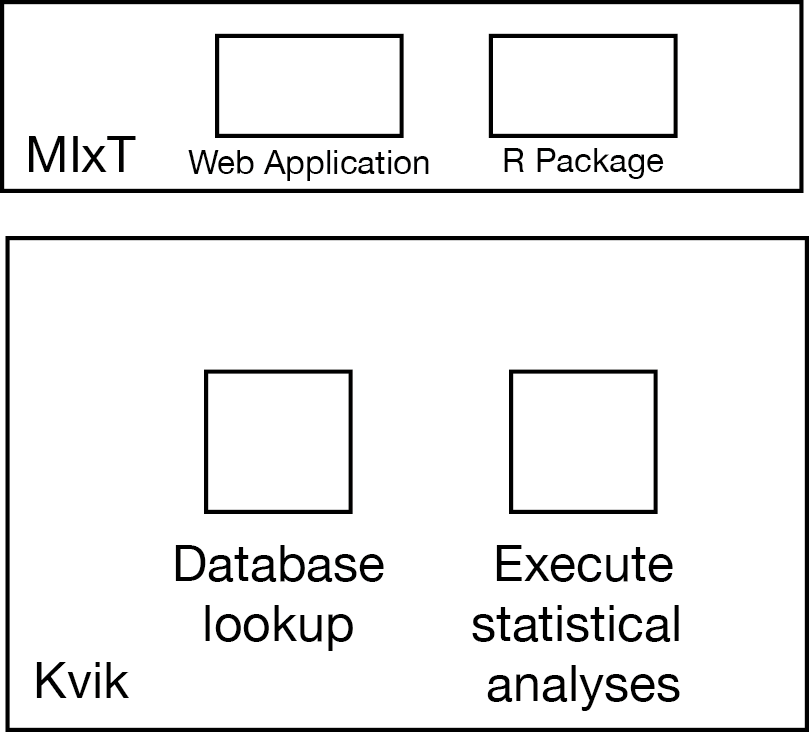
\includegraphics{figures/kvik-mixt.png}
\caption{An overview of the relationship between the MIxT application and Kvik.
MIxT contains a web application (online at \url{mixt-blood-tumor.bci.mcgill.ca})
and the R Package that provides analyses and data to the web application. Kvik
provides the services for running the statistical analyses from the R package,
and the database lookups found in the web application.} 
\label{kvik-mixt}
\end{figure} 

